\section*{Decay Time Distibrution}
In the last section of the experiment, the study of the decay timing distribution is presented.
The timing distribution was produced, for both the decay channel, with a TAC unit using as start the  fourth detector, vertically mounted over the source, and as stop the coincidence between it and the detectors on the rotating arms (two or three depending on the decay channel). 
The obtained distribution are shown in Fig.~\ref{Fig:DecayDist}.

\begin{figure}[H]
	\centering
	\subfloat[][\emph{p-Ps}.]
	{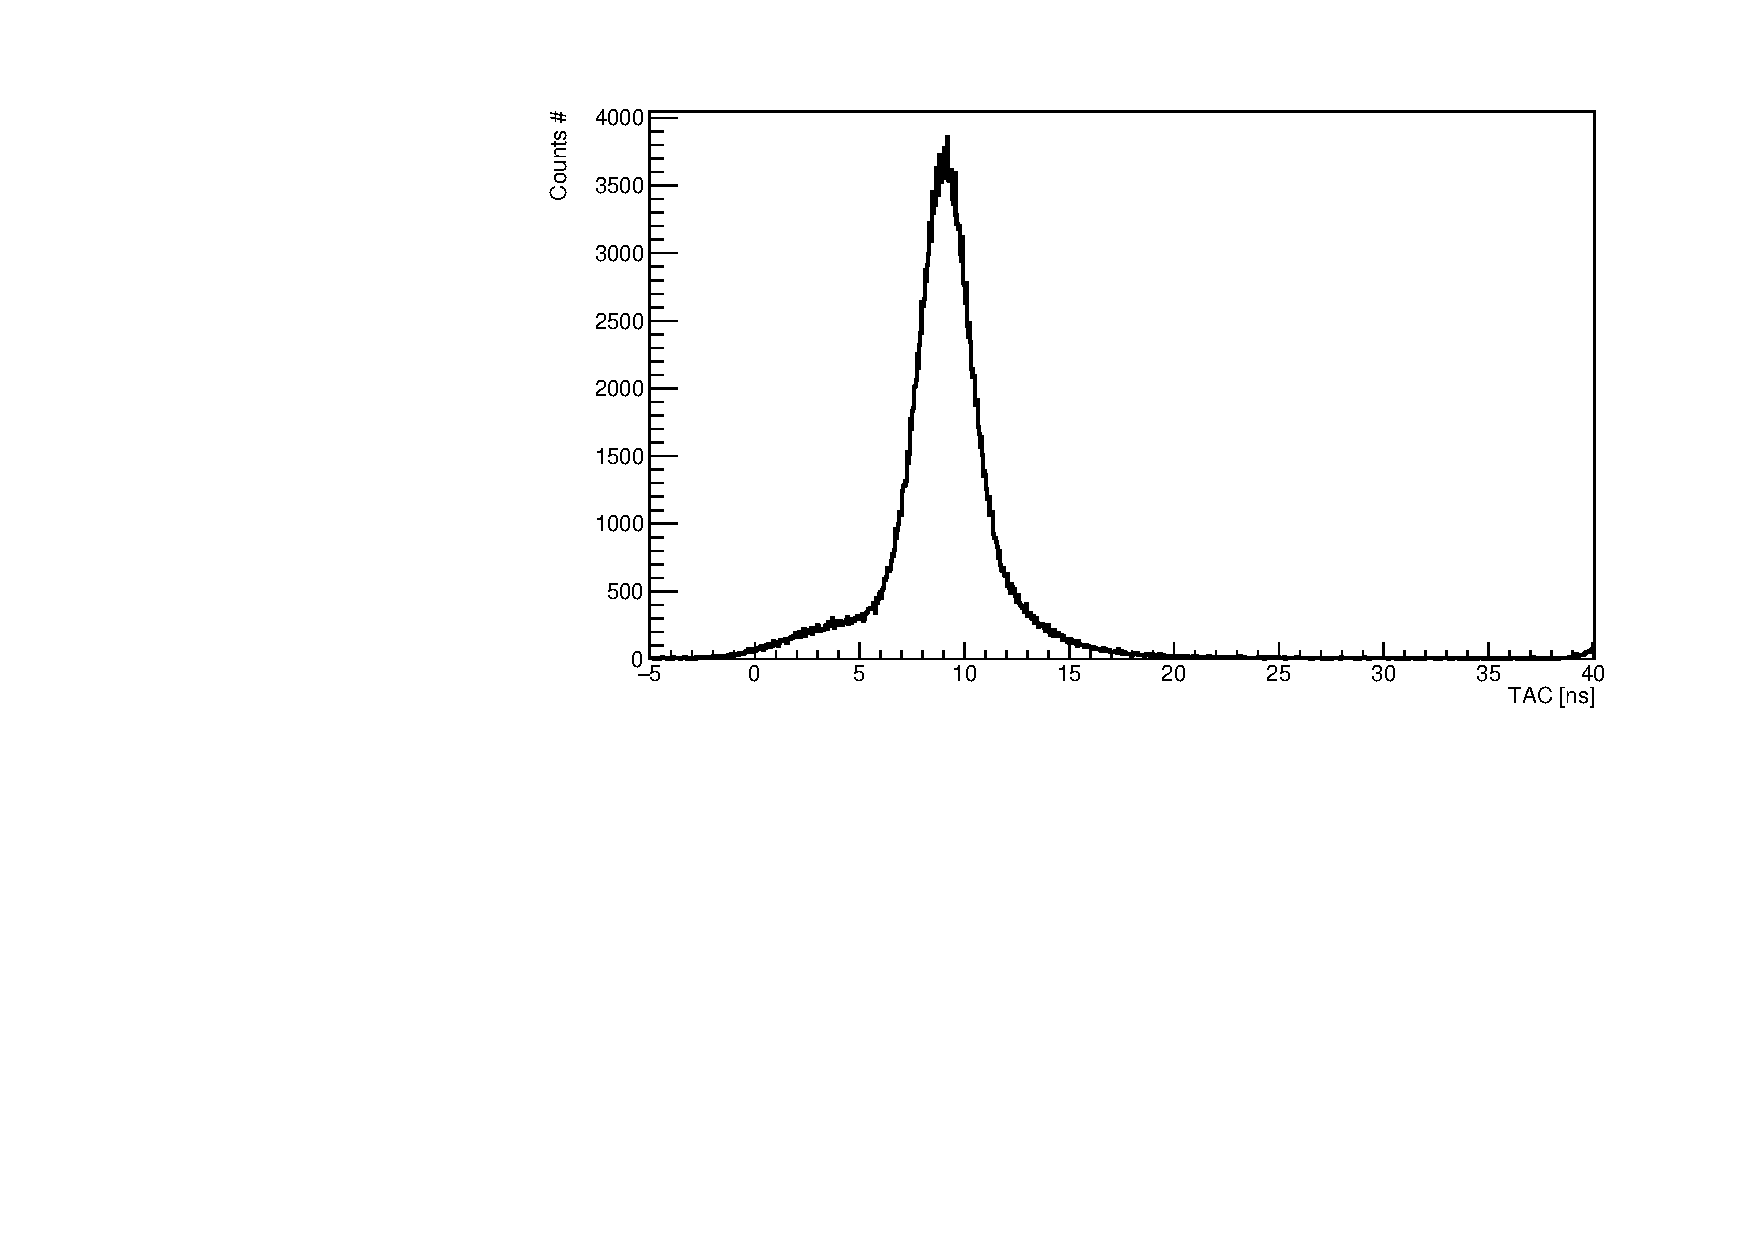
\includegraphics[width=.45\textwidth]{1_2_TAC_ch3}} \quad
		\subfloat[][\emph{o-Ps}.]
	{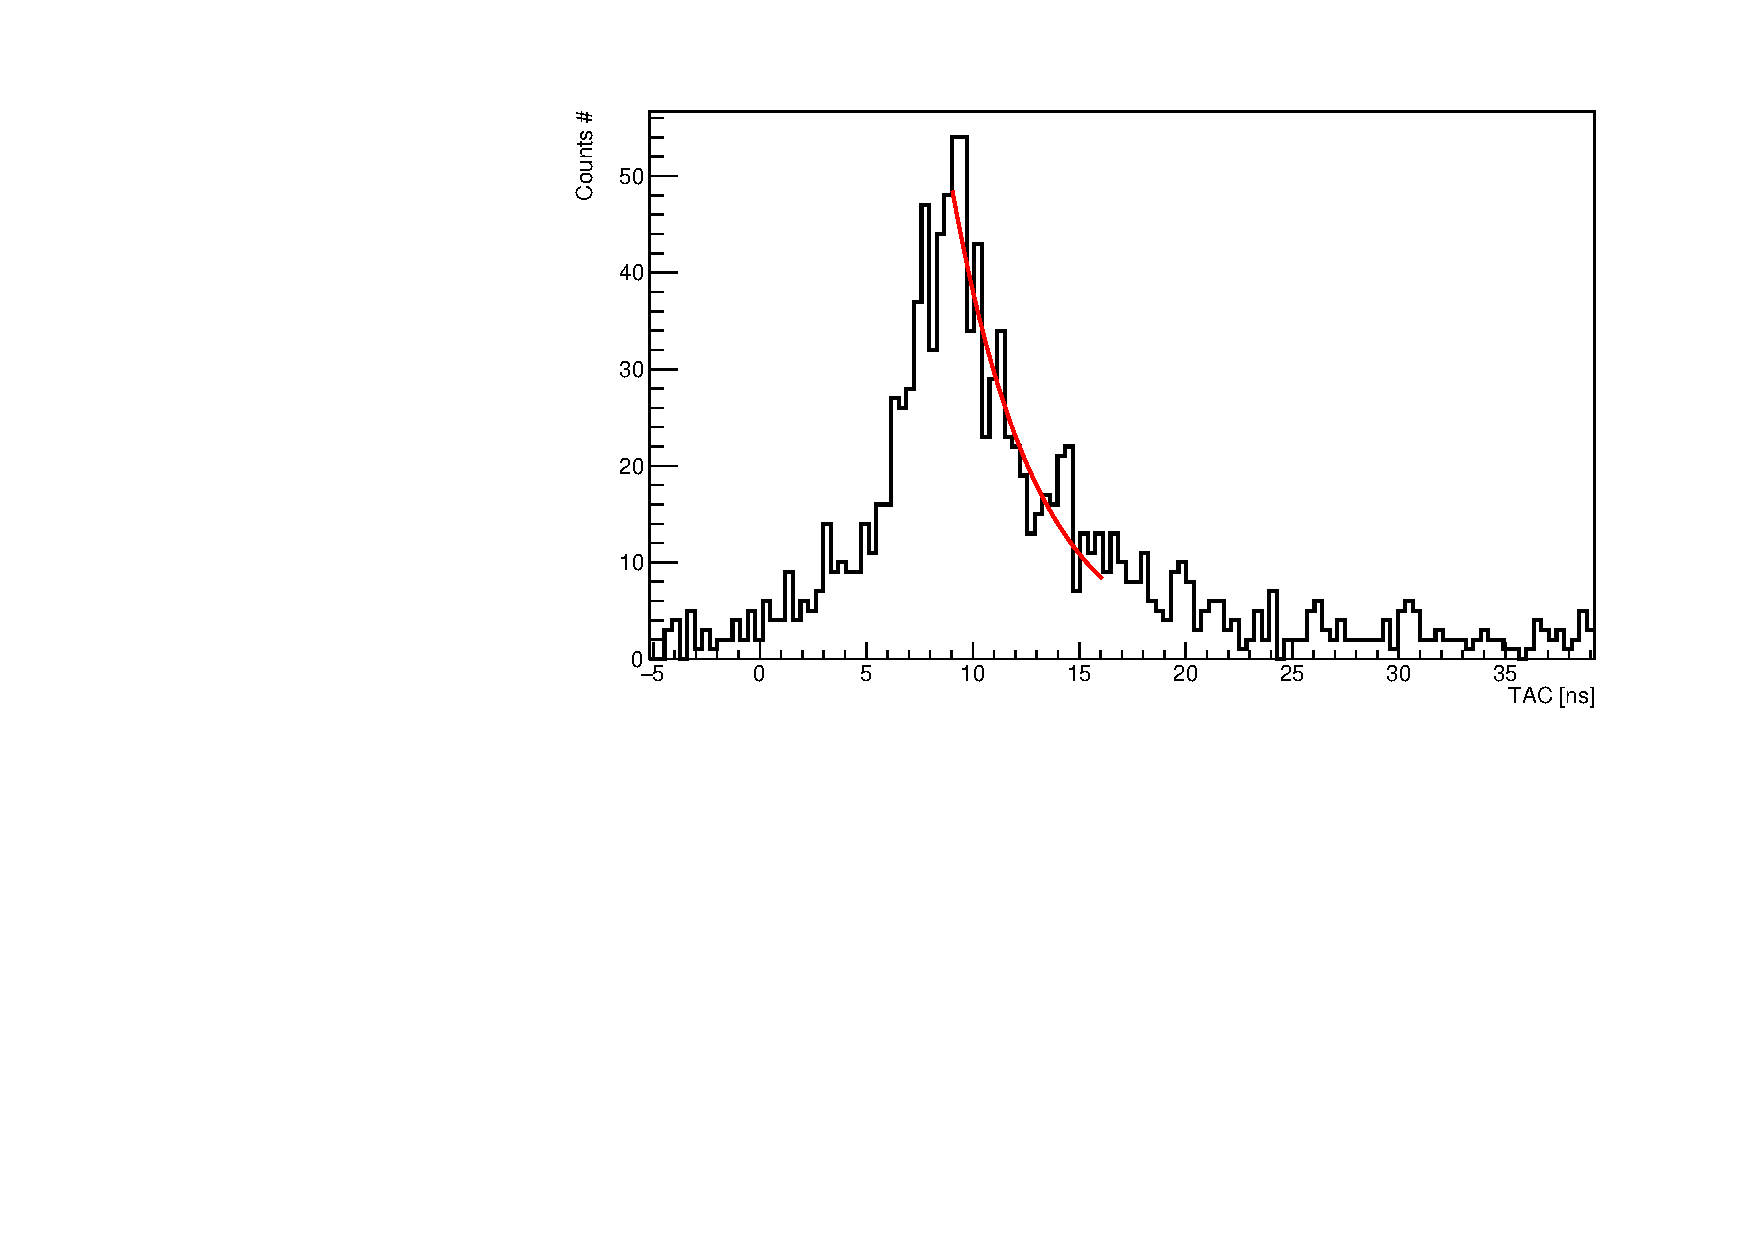
\includegraphics[width=.45\textwidth]{1_2_3_TAC_ch3_fitted}} \\
	\caption{Decay time distribution obtained selecting (\emph{a}) p-Ps and (\emph{b}) o-Ps channel. }
    \label{Fig:DecayDist}
\end{figure}

In the case of o-Ps, an exponential fit over the right tail of the distribution was performed in order to give an estimate of the decay constant. The slope ($1/\tau$) resulted $(2.5 \pm0.2)\times 10^{-1}$~$1/$ns, i.e. $\tau = 4.0\pm0.4$~ns, definitely too far from the 142~ns lifetime. This difference is mainly due to the low statistic of o-Ps decay.

The decay constant estimation was not performed in the case of p-Ps, which have a lifetime of  0.125~ns, too small to be measured with the setup used.
